\TODO
Unconventional computation.
Bio-inspired design methods.
EHW: Evolvable hardware.
POE: Phylogeny, Ontogeny, Epigenesis \cite{sipper1997poe}.

Features: Graceful degradation, Robustness, Redundancy.

\TODO
Phylogeny, named after evolution of the species "Phylogeny" is temporal evolution due to mutation, reproduction.
Provides diverity for "survival of the fittest".
Ontogeny = development / cell division, a zygote replicates into a larger structure where each cell specializes.
Difficult to store each cell type/function.
Example: Human brain can't be specified by genome.
Epigenesis: Modification (learning) during the lifetime of the organism.

\TODO
Equivalent: Artificial Evolution, Artificial Development, Artificial Learning.
The two first are used in this thesis.

%==============================================================================%

\section{Evolution}

Evolution is the natural process that over time advances species by letting the fit survive and the weak perish.
Essentially, each generation tries slight variations to try to gradually create a species that is more fitting to the environment, in effect creating a better solution to the problem of life.

Similarly, artificial evolution can be used by computers to evolve solutions instead of manually creating them.
Evolutionary Algorithms (EAs) can search millions of possible solutions, guided by their fitness scores, and find solutions that humans would never have imagined.
In contrast to nature, where years usually pass between generations, powerful computers can create hundreds of generations every second and find good solutions in relative short time.

EAs have been successfully applied to many scientific tasks.
For example, NASA has had great success with evolving antenna designs \cite{hornby2006antenna}, and Haddow and Tufte have evolved robot controllers \cite{haddow1999robot}.

\subsection{Genetic Algorithms}

A Genetic Algorithm (GA) is a very common type of EA.
It represents each solution as a genotype, a binary string used as a blueprint to create the solution itself, called a phenotype.
The genotype is comparable to nature's DNA, and it is this genetic material which is modified in the evolutionary process.

\begin{figure}[!ht]
    \centering
    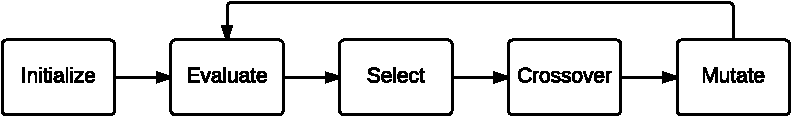
\includegraphics[width=0.85\textwidth]{ga}
    \caption[Genetic Algorithm]{
        A genetic algorithm.
        The cycle is broken when the fitness is above a given threshold.
    }
    \label{fig:ga}
\end{figure}

The GA process is shown in \figurename~\ref{fig:ga}.
First, a base population with random genotypes is generated.
Then, each phenotype is constructed and evaluated using a fitness function.
If a solution has a fitness score above a set threshold, the process stops.
Otherwise, a new population is created by selecting solutions with high fitness scores, crossing their genotypes, and mutating the results, before repeating the process.

%==============================================================================%

\section{Development}

The process that transforms a genotype into a phenotype is called development.
It can be regarded as a form of decompression algorithm \cite{harding2008artificial}.
In nature, this process is seen when a single cell transforms into a more complex multicellular organism, as visualized in \figurename~\ref{fig:development}.
Unlike with a pure decompression algorithm however, biological systems also use information about their environments to tailor themselves to them.
This is known as plasticity.

\begin{figure}[!ht]
    \centering
    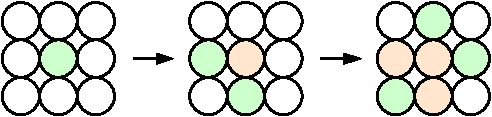
\includegraphics[width=0.5\textwidth]{development}
    \caption[Development]{
        Example of cells replicating and changing to develop a larger entity.
        \todo{use actual ca figs?}
    }
    \label{fig:development}
\end{figure}

Development is needed because a complete specification of a complex organism requires much more information than practically can be stored; it is several orders of magnitude greater than that of one cell and it's development rules.
Plasticity and self-repairing abilities are merely bonuses, but have shown to be highly valuable properties.
For the same reasons, artificial development is lucrative for building more complex computer systems that is also fault-tolerant and adaptable.

Development is never necessarily ``finished''; it can continue during the entire lifespan of the system.
\todo{explain attractors}
The system will eventually end up in cycle or point attractors, but external variables will likely cause it to break from it and follow a different path.

\subsection{Lindenmayer Systems}

Perhaps the most known and widely used artificial development systems are Lindenmayer Systems (L-Systems).
It was introduced by biologist and botanist Lindenmayer in 1968 to describe the growth of plants and fungi \cite{lindenmayer1968models}.
The L-System is a form of parallel generative grammar; starting with an axiom, a string is built by iteratively applying all the grammar rules in parallel.
The string is a representation of the structure of the object.
Each character symbolizes a branch, twist, turn, stretch or other feature.

\begin{figure}[!ht]
    \centering
    \begin{subfigure}{0.32\textwidth}
        \centering
        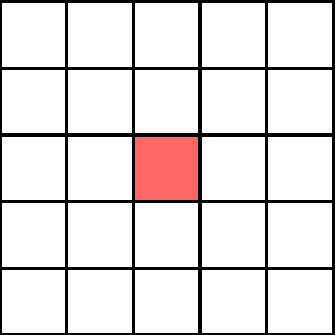
\includegraphics[width=0.9\textwidth]{dragon/00}
        \caption{Iteration 0}
    \end{subfigure}
    \begin{subfigure}{0.32\textwidth}
        \centering
        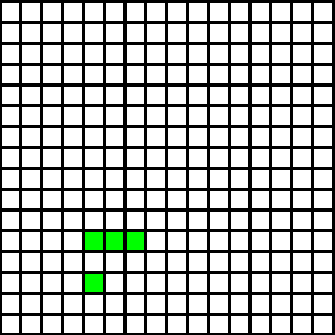
\includegraphics[width=0.9\textwidth]{dragon/02}
        \caption{Iteration 2}
    \end{subfigure}
    \begin{subfigure}{0.32\textwidth}
        \centering
        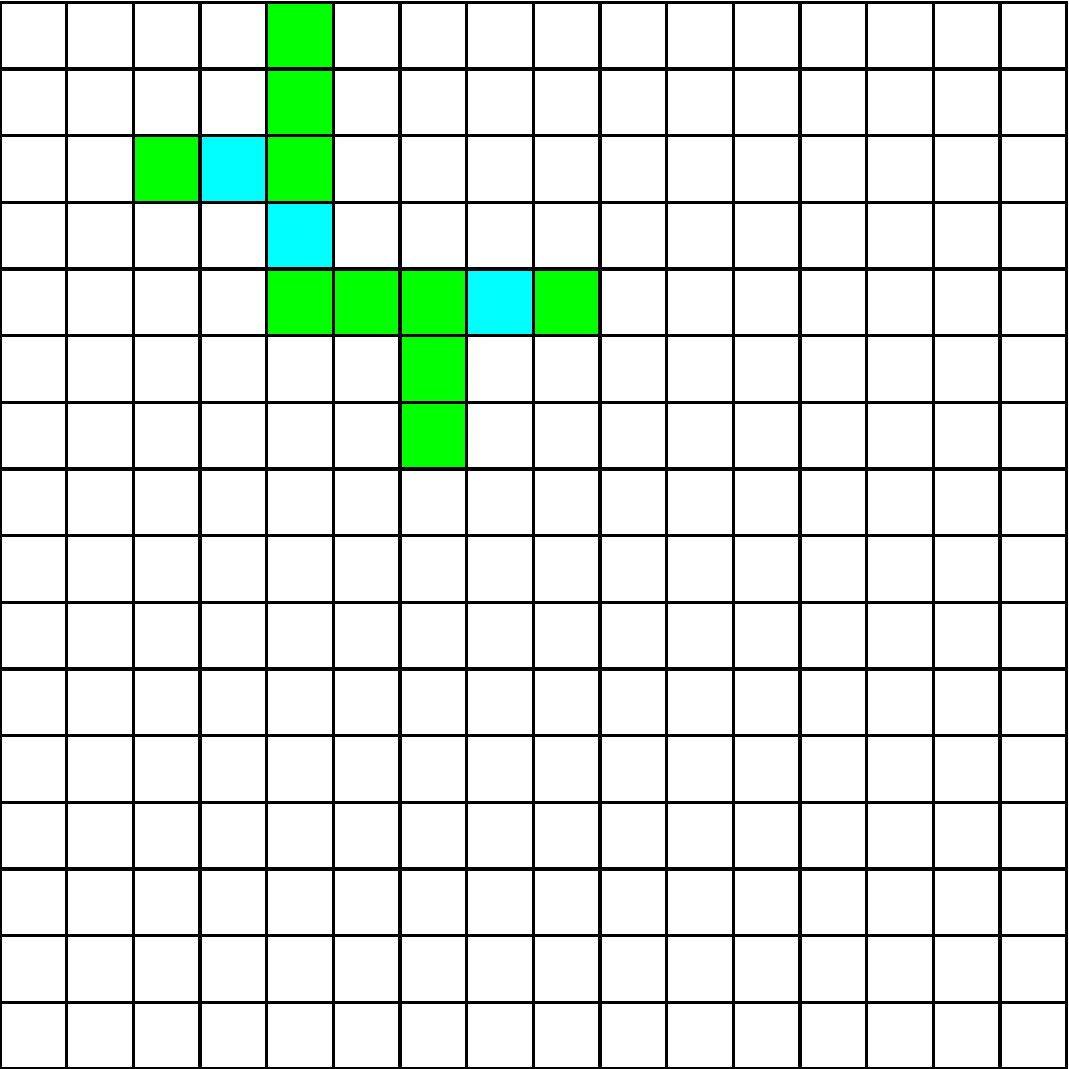
\includegraphics[width=0.9\textwidth]{dragon/04}
        \caption{Iteration 4}
    \end{subfigure}
    \par\bigskip
    \begin{subfigure}{0.32\textwidth}
        \centering
        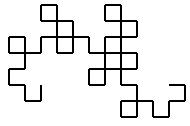
\includegraphics[width=0.9\textwidth]{dragon/06}
        \caption{Iteration 6}
    \end{subfigure}
    \begin{subfigure}{0.32\textwidth}
        \centering
        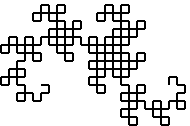
\includegraphics[width=0.9\textwidth]{dragon/08}
        \caption{Iteration 8}
    \end{subfigure}
    \begin{subfigure}{0.32\textwidth}
        \centering
        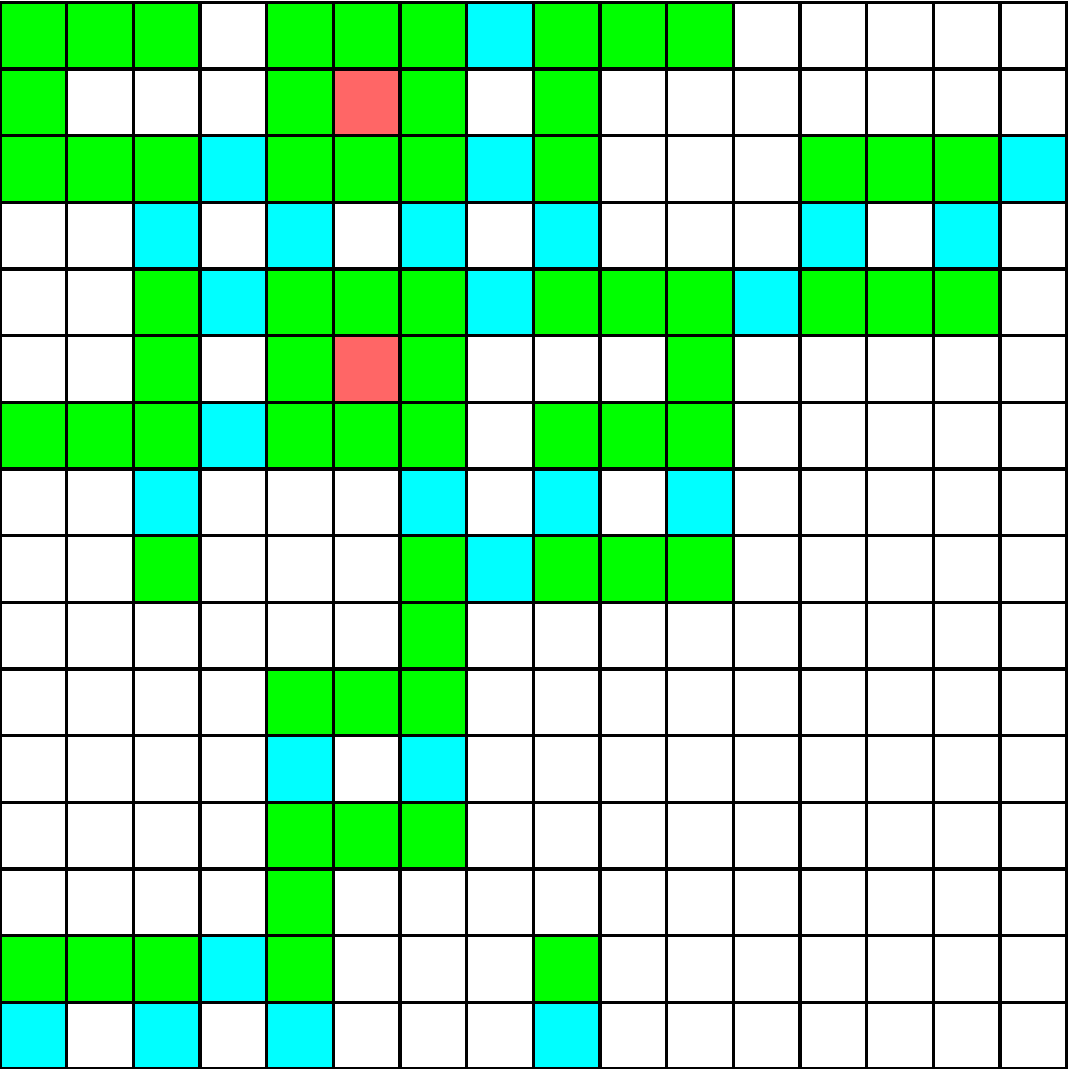
\includegraphics[width=0.9\textwidth]{dragon/10}
        \caption{Iteration 10}
    \end{subfigure}
    \caption[Dragon curve]{
        Heighway dragon curve generated with L-System using \cite{lsystemgenerator}.
        The starting string is $FX$ and the rules are $X \rightarrow XRYFR$ and $Y \rightarrow LFXLY$ where $F$ is forward, $R$ is a right turn and $L$ is a left turn\footnotemark.
    }
    \label{fig:dragon-curve}
\end{figure}

\footnotetext{
    \cite{lsystemgenerator} uses $+$, $-$ and a customizable angle instead of $L$ and $R$.
}

In addition to plants, L-Systems are also suitable for generating other structures that grow and branch.
\figurename~\ref{fig:dragon-curve} shows how they can be used to generate fractals, specifically the dragon curve \cite{gardner1967heighway}.
It is the pattern that emerges when a piece of paper is folded many times and then each fold is opened to a 90 degree angle.
The corresponding L-System uses only two rules, and is a testament to how very simple development rules can create outstandingly complex shapes.
L-Systems have also been applied to other tasks, such as music composition \cite{manousakis2006musical}.

%==============================================================================%

\section{Evolution in Materio}

\TODO
Embodiment principles.
Evolve in software, test in software.
Evolve in software, test in hardware.
Evolve and test in hardware.

%==============================================================================%

\section{Cellular Automata}

A Cellular Automaton (CA) is a computational structure made up of vast numbers of very simple functional elements called cells that are arranged in a grid.
Each cell contains a state and is connected to a handful of nearby cells to form neighborhoods.
\todo{fig?}
At given time intervals the cells then update their states based on a transfer function over the states in their neighborhoods.\footnotemark

\footnotetext{
    CAs are specific cases of Random Boolean Networks \cite{gershenson2004rbn}.
}

CAs are attempts to mimic the structures found in biological lifeforms, where complex results emerge from interactions between many simple cells.
The key principles are massive parallelism, local interactions and simple computational units.
As seen in \figurename~\ref{fig:computing-principles}, this is the direct opposite paradigm of the general-purpose serial architecture that is common in computers today.
However, CAs have been shown to be Turing complete \cite{codd1968cellular, neumann1966selfreplication}, and can therefore perform the same tasks.

\begin{figure}[!ht]
    \centering
    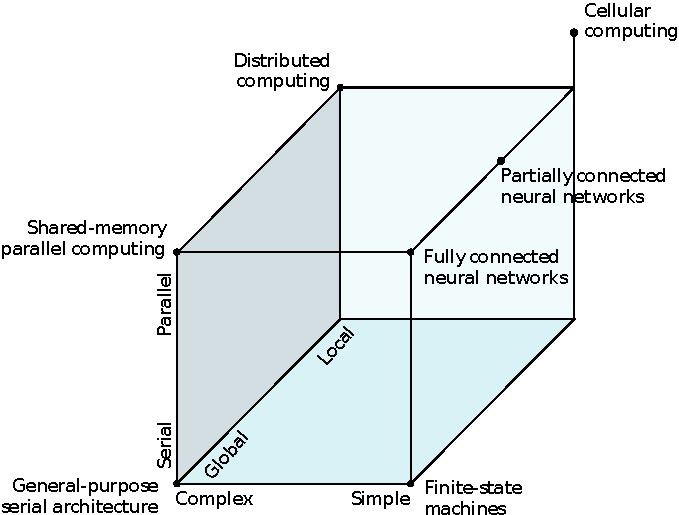
\includegraphics[width=0.82\textwidth]{computing-principles}
    \caption[Computing principles]{
        Graphical representation of how different computing paradigms relate with regards to computing principles.
        (Reprinted from \cite{sipper1999emergence})
    }
    \label{fig:computing-principles}
\end{figure}

CAs are attractive due to their inherent robustness and scalability when paired with development.
In the event of broken cells, signals can simply be rerouted, and to increase the performance, extra cells can be added and the program grown; local communication ensures that there are no bottlenecks.
This greatly contrasts modern processors where a broken part normally renders the entire chip unusable, and adding more cores are of limited benefit due to the shared-memory architecture.
Increasing the clock rate is no longer an option either, due to the fixed power budget \cn{tdt1?}.

A major challenge with CAs is programming.
CAs compute by emergence using massive parallelism, while humans mostly solve problems serially \cite{newell1972problemsolving}.
This makes it near impossible for humans to construct programs, unless for very simple problems.
Genetic Algorithms are therefore often used.

Other major challenges are the representation of input and parsing of output.
Both arise due to the CA's distributed nature.
One possibility for input is \todo{example or remove}.
For output, the Discrete Fourier Transform (DFT) over the number of cells with a given state appears promising \cite{berg2013ca}.

CAs have been also been used in various research.
They have been the environments for simulating lifeforms and creating replicating machines \cite{neumann1966selfreplication}.
A very popular life simulator is Conway's Game of Life \cite{gardner1970life}.
\todo{move me maybe?}

There are many variations of CAs, which are discussed in great detail in \cite{sipper1999emergence}.
Following is a brief summary:
Cell states can be discrete or continuous values.
The transfer function can be represented by exhaustive enumeration or a parameterized expression.
The cells may be uniform by having the same transfer function, or non-uniform.
Cell updates can be synchronous or asynchronous, and in the latter case the CA can be either deterministic or non-deterministic depending on the order in which cells update.
The CA may be fully specified by direct programming or adaptively evolved using a GA or similar.
Finally, there are numerous schemes that can be used to connect cells together to form neighborhoods.

Only a specific form of CA is used in this thesis:
Discrete, exhaustively enumerated, non-uniform, synchronous and deterministic.
It is possible to use direct programming, but there are systems in place for adaptive evolution.

\subsection{Neighborhoods}

An important property of CAs is how cells are connected to form neighborhoods, as this defines what data will be available for the transfer functions and therefore changes the way data flows through the machine.
It is common to connect directly adjacent cells, and sometimes those diagonally adjacent.
Cells do not have to be part of their own neighborhoods, but it is common to have them be so.
The von Neumann neighborhood shown in \figurename~\ref{fig:neighborhood} is commonly used for 2D CAs, and is also used by the design in this thesis.
It includes the directly adjacent cells; north, south, east and west; and the cell itself.

\begin{figure}[!ht]
    \centering
    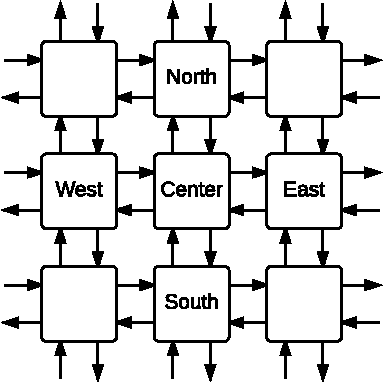
\includegraphics[width=0.42\textwidth]{neighborhood}
    \caption[von Neumann Neighborhood]{
        The von Neumann neighborhood in a 2D CA.
        The cell states are shared with all directly adjacent cells.
    }
    \label{fig:neighborhood}
\end{figure}

The von Neumann neighborhood is easily extendable to 3D by adding the cells directly above and below to the neighborhood.
The extra dimension allow more complex signal routing since the signals can cross over or under each other, which hopefully allow more complex computation.
It should however be possible to achieve the same complexity in fewer dimensions by increasing the neighborhood size \CN, but that would require more advanced transfer functions.

\subsection{Complexity Classes}

Wolfram observed that some CAs developed complex pattern while others decayed into uniformity or chaos.
He therefore developed a set of four classes to group them based on their emergent behavior \cite{wolfram1984complexity}:

\begin{itemize}
    \item Class 1 – Uniform:
        The CA quickly results in a homogeneous state, regardless of initial condition.
        It lacks the means to store data, as well as perform computation.
    \item Class 2 – Repetitive:
        The CA develops both periodic and static data structures.
        However, after a number of cycles the states begin to repeat.
        This makes complex computation impossible.
    \item Class 3 – Chaotic:
        The CA is not held back by repetition as with class 2, but the patterns are so chaotic that it is unable to support data structures.
    \item Class 4 – Complex:
        The CA supports complex data structures and has no discernible repetition.
        It should be capable of universal computation.
\end{itemize}

\begin{figure}[!ht]
    \centering
    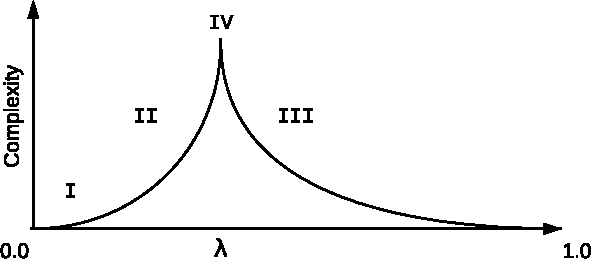
\includegraphics[width=0.66\textwidth]{complexity-classes}
    \caption[Complexity classes]{
        The location of Wolframs complexity classes in $\lambda$ space.
        (Adapted reprint from \cite{langton1990edgeofchaos})
    }
    \label{fig:complexity-classes}
\end{figure}

Langton attempted to connect Wolframs classes to CA rule complexity \cite{langton1990edgeofchaos}.
For this he used a measure called $\lambda$, which essentially determines the inverse ratio of rules that cause a cell to transition into any given state.
%This means that all transitions are to a given state if $\lambda=0.0$, while there are none if $\lambda=1.0$.
His findings, displayed in \figurename~\ref{fig:complexity-classes}, show that class 4 resides in a phase transition between the order of class 2 and the chaos of class 3.
This is known as ``The Edge of Chaos''.

\subsection{Evolution and Development}

\TODO
CA + Dev + GA = True.
GA to find development rules.
Development used to create CA structure.
CA can then be run to perform computation.
Moore's law.
\figurename~\ref{fig:evo-devo-ca}.

\begin{figure}[!ht]
    \centering
    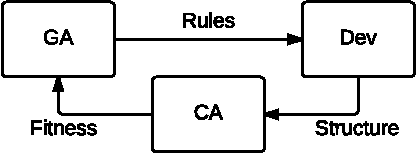
\includegraphics[width=0.44\textwidth]{evo-devo-ca}
    \caption[CA system with evolution and development]{
        Example CA system with evolution and development.
    }
    \label{fig:evo-devo-ca}
\end{figure}

%==============================================================================%

\section{FPGA}

A Field Programmable Gate Array (FPGA) is a type of reconfigurable hardware.
It can implement any desired logical operation by configuring and connecting a number of lookup tables (LUTs) and flip-flops (FFs).
FPGAs can also contain dedicated blocks for addition, multiplication, storage, and other functions.
The resources are grouped into configurable logic blocks (CLBs), which through a network of interconnects can be connected to each other or input/output pins.
An example of this structure is shown in \figurename~\ref{fig:fpga}.
Note that modern FPGAs consists of thousands of CLBs and hundreds of I/O pins \cite{ds160}.

\begin{figure}[!ht]
    \centering
    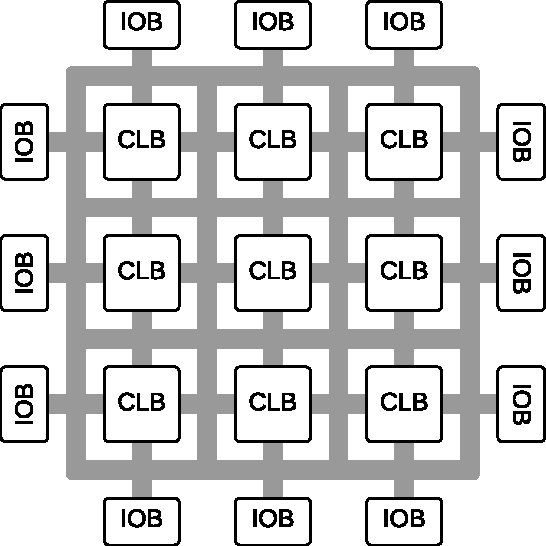
\includegraphics[width=0.55\textwidth]{fpga}
    \caption[FPGA]{
        High-level block diagram of an FPGA.
        An array of configurable logic blocks (CLBs) and input/output blocks (IOBs) are connected by a network of interconnects.
    }
    \label{fig:fpga}
\end{figure}

FPGAs have been the subject of EHW research due to their reconfigurability, and several researchers have been successful in evolving working electronic circuits \cite{huelsbergen1998evolution, thompson1997evolved}.
However, the resulting circuits have often ended up using intrinsic properties of the silicon and been very sensitive to environmental changes.
A problem with using modern FPGAs is that some configuration bit strings can destroy the FPGA by creating short-circuits \cite{xapp151, ug380}.
This means that the bit strings can not be used directly as the genotype without complicated tests to discard those that are dangerous.

The regular structure of an FPGA makes it well suited as the basis for implementing CAs however, especially those that are 2D.
\todo{more?}

\subsection{Sblock}
\label{sec:sblock}

The sblock was introduced as part of a new EHW-friendly FPGA architecture in \cite{haddow2000sblock}.
The architecture is a non-uniform CA with a von Neumann neighborhood, where the update function of each cell is independently configurable at run-time.
The cells, known as sblocks, are very simple structures; they consist of a configurable LUT and a FF, as shown in \figurename~\ref{fig:sblock}.

\begin{figure}[!ht]
    \centering
    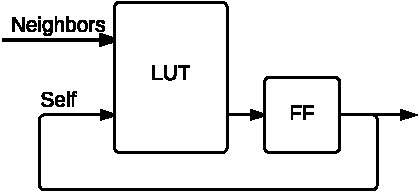
\includegraphics[width=0.44\textwidth]{sblock}
    \caption[Sblock]{
        Detailed block diagram of an sblock.
        The LUT can be reconfigured on-the-fly to implement any logical function.
    }
    \label{fig:sblock}
\end{figure}

The greatest benefit of using sblocks for EHW research is that there is no risk of damage or exploitation of intrinsic properties in the silicon.
Additionally, the simple structure and hardwired signal routing allows for very efficient area usage.
The likelihood of a mass-produced sblock-FPGA arriving on the market in the near future is slim.
However, it is possible to implement it virtually within another FPGA, as in this thesis.

%==============================================================================%

\section{PCI Express}

The PCI Express interface was designed to tackle the arising trouble with clocked parallel buses like PCI.
The problem with such buses is that the clock speed can not be increased beyond a given threshold, as the slightly different lengths of the wires causes data to arrive at slightly different times.
Reducing the clock period to less than the variation in arrival time means the data will become corrupted.
This problem is exacerbated with increasing bus size.

PCI Express is therefore based on serial communication over differential pairs (lanes\footnotemark) without the need for a reference clock \cite{pcie}.
\footnotetext{
    PCI Express operates in full duplex mode, which means that each lane has an independent differential pair in each direction.
    1, 2, 4, 8, 16 or 32 lanes are supported, but data is striped and thus still transmitted serially.
}
This allows an extremely fast clock speed compared to a parallel bus, and much greater bandwidth in total.
PCI Express consists of three layers; the physical layer, the data link layer and the transaction layer, structured as shown in \figurename~\ref{fig:pcie}.

\begin{figure}[!ht]
    \centering
    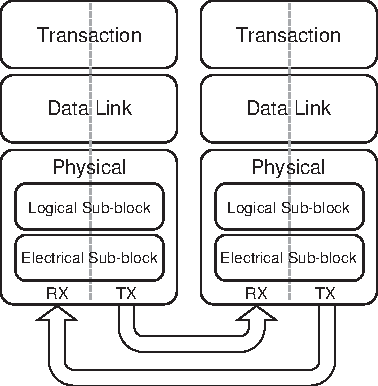
\includegraphics[width=0.46\textwidth]{pcie}
    \caption[PCI Express structure]{
        High-level diagram showing the layered structure of PCI Express. (Reprinted from \cite{pcie})
    }
    \label{fig:pcie}
\end{figure}

The transaction layer's primary responsibility is the creation and parsing of transaction layer packets (TLPs).
TLPs are used to trigger events or start various transactions, most commonly to initiate read and write requests\footnotemark.
\footnotetext{
    Read and write requests are directed at one of up to six base address registers (BARs).
    They represent internal memory areas that can be anywhere from a few bytes to several gigabytes in size.
}
Most requests entail the return of a completion TLP containing the requested data or other information.
TLPs consists of multiple 32-bit double words (DW), where the first is a common header describing the type of packet.

The data link layer ensures integrity by adding error detection codes to outgoing TLPs and performing error detection and correction on incoming TLPs.
It is also responsible for retransmission if corruption occurs.

The physical layer is responsible for serialization and deserialization of the data stream.
Each byte is padded with two extra bits (8b/10b encoding) to allow clock recovery.

%==============================================================================%

\section{Related Work}

This section describes work performed by others, which is related to that performed in this thesis.

% Format: Who? What? When? Main feature? Relation?

\subsection{CAM-8}

The Information Mechanics Group at MIT Laboratory for Computer Science has had a focus the question ``How can computation and computers best be adapted to the constraints and opportunities afforded my microscopic physics?''
This has led to more than a decade of study of CAs, as their fine-grained computation with local interconnectivity are particularly good candidates for micro-physical efficiency.
To this end, they have created CA Machines (CAMs) that aim to use common computer parts in smart arrangements to provide CA computation performance akin to modern supercomputers.
\cite{margolus1996cam8} describes their eighth iteration, known as the CAM-8.

\begin{figure}[!ht]
    \centering
    \begin{subfigure}{0.48\textwidth}
        \centering
        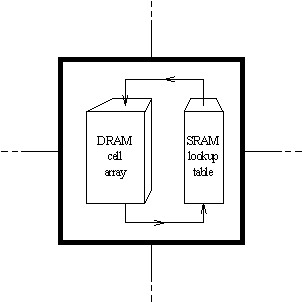
\includegraphics[width=0.9\textwidth]{cam8-a}
        \caption{A single processing node}
    \end{subfigure}
    \begin{subfigure}{0.48\textwidth}
        \centering
        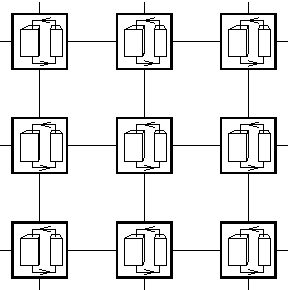
\includegraphics[width=0.9\textwidth]{cam8-b}
        \caption{Spatial array of CAM-8 nodes}
    \end{subfigure}
    \caption[CAM-8 system diagram]{
        CAM-8 system diagram.
        (Reprinted from \cite{margolus1996cam8})
    }
    \label{fig:cam-8}
\end{figure}

The CAM-8 implements a discrete, exhaustively enumerated, uniform, and synchronous 3D CA split over multiple nodes that run in parallel.
Any number of nodes can be connected to form a CA of desired size, and an 8-module prototype showed to be on par with regular supercomputer simulations.
As illustrated in \figurename~\ref{fig:cam-8}, each node contains DRAM that potentially holds millions of cells and an SRAM that holds the LUT for the current program.
Within each node, cells are updated in sequence, making it a semi-parallel machine.
This is a trade-off that compromises performance for the benefit of massively increased CA size and the ability to use common hardware.
For 1-bit cell states, the prototype is capable of $3 \cdot 10^9$ cell updates per second and can fit up to $5 \cdot 10^8$ cells.

\todo{Maybe}
The lookup table can be exchanged for a pipelined function.
Instead of traditional fixed neighborhoods, CAM-8 uses advanced bit-shifting techniques to collect neighborhood data from the DRAM.
Each node is connected to the front-end workstation through a tree network.
Problem: Must encode computation into uniform and local spatial matrix.
Harness the astronomical computing power that is available in CA format

\subsection{CAM-Brain Machine}

In \cite{degaris2001cbm}, de Garis et al. introduces the CAM-Brain Machine (CBM), an FPGA-based platform that implements a CA-based neural network that is evolved using a GA.
It is part of de Garis' ``Artificial Brain Project'', which goal is to build an artificial brain with 1 billion neurons.
The CBM is a stepping stone in the right direction, and allows the formation an artificial brain with nearly 75 million neurons in a CA of 843 million cells that is split across 64640 modules.

The CBM implements the Collect and Distribute (CoDi) based neural network model from \cite{gers1998codi}, which goal is to accelerate brain evolution and simulation speeds by a factor of 500 compared to CAM-8, to facilitate the higher update speeds required for real-time control of a robot.
It is a 3D CA with four cell types: Neurons, axons, dendrites and empty.
Neurons essentially perform a threshold function over their inputs, while axons carry the neural signals to other neurons, and dendrites consolidate the signals from multiple axons.
The CA is initialized with evenly spaced neurons, and then developed by alternately growing axons and dendrites from the neurons.
Which cells grow axons or dendrites are determined by artificial evolution.

Brain building is still mostly in the ``proof of concept'' phase, so to attract attention to further research they designed a cute life-sized robot kitten that would be controlled by the CBM.
The work to design and evolve it's brain architecture was expected to continue well into the 2000s, but was halted when the research institution went bankrupt in 2001 \cite{giles2001utopian}.

\subsection{Firefly}

\TODO
Moshe Zipper: Evolution of Parallel Cellular Machines

\subsection{BioWall}

\TODO
Focuses on the ontogenetic axis through embryonics.
Machine that displayes the principles of embryonics to the public through visual and tactile interactions.
5.3 meters wide.
Supports 2D cellular systems: CAs or Neural nets.
Limitless possibilities.
Main example:
BioWatch.
Other examples:
Game of Life.
Replicating structures.
von Neumann's universal constructor.

\begin{figure}[!ht]
    \centering
    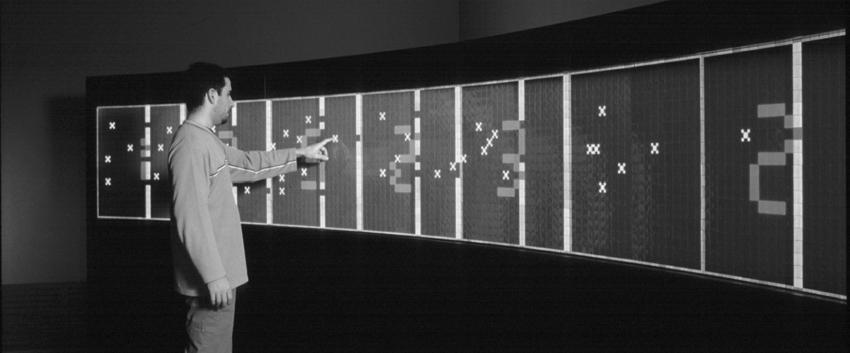
\includegraphics[width=\textwidth]{biowall}
    \caption[BioWall]{
        The BioWall running BioWatch.
        (Reprinted from \cite{tempesti2002biowall})
    }
    \label{fig:cam-8}
\end{figure}
